% ---------------------------------------------------------------------------
% Figure 1 -- the grid as a signed heat map. This is what \ref{fig:grid} in the
% Introduction points at.
%
% Spans both columns, so figure* and not figure. Put it anywhere in the
% Introduction; LaTeX floats it to the top of a page by itself.
%
% Needs \usepackage{graphicx} in the preamble, which the IEEE template loads.
% Upload paper/fig_grid.pdf to Overleaf alongside main.tex. Use the PDF and not
% the PNG, since the PDF is vector and stays sharp at any size.
%
% Regenerate with experiments/make_grid_figure.py, which recomputes every cell
% from the episode records through the same paired() the report uses. Do not
% edit the numbers here, because there are none to edit.
% ---------------------------------------------------------------------------

\begin{figure*}[t]
\centering
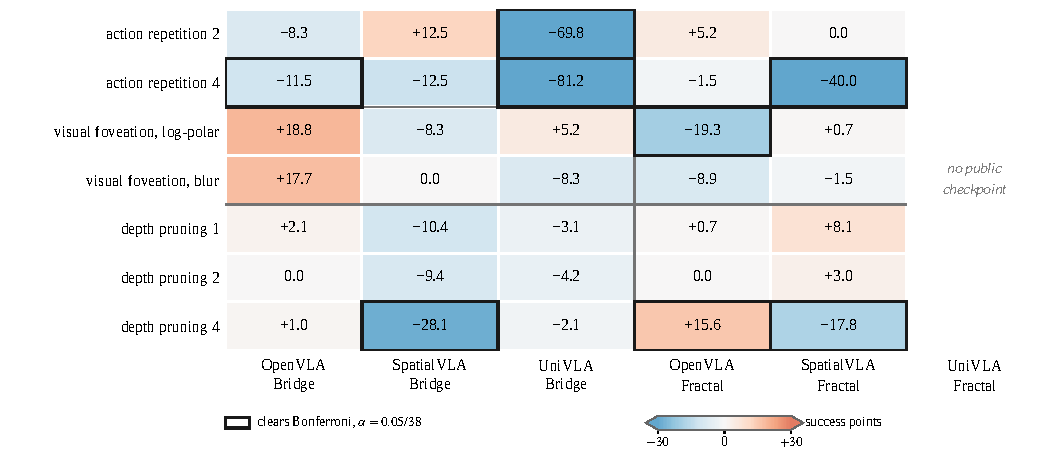
\includegraphics[width=\textwidth]{fig_grid.pdf}
\caption{Every condition in the grid, as the paired change in success against
that cell's own baseline. Positive is red and negative is blue. A cell pairs
only the episodes present in both runs, and a box marks the eight cells that
clear a Bonferroni threshold of $\alpha = 0.05/38$ over the paired tests the
grid runs. The scale is clipped at $\pm 30$ points so that the cells carrying
an argument stay legible, and the three cells past it keep their printed
value. Read along any row. The same intervention, applied the same way, moves
in both directions depending only on which cell it was measured in, and the
bottom row does so with both directions individually significant.}
\label{fig:grid}
\end{figure*}
